\documentclass{article}

\usepackage[a4paper, top=3cm, left=3cm, right=3cm, bottom=3cm]{geometry}
\usepackage{graphicx}
\usepackage{lmodern}
\usepackage{lscape}

\renewcommand{\thesection}{}
\renewcommand{\thesubsection}{\arabic{subsection}}

\title{Fonctionnalit\'es Projet}
\author{Kevin Alary \& Nicolas Yon}
\date{}


\begin{document}

\maketitle

\section{DDD(Domain driven design)}
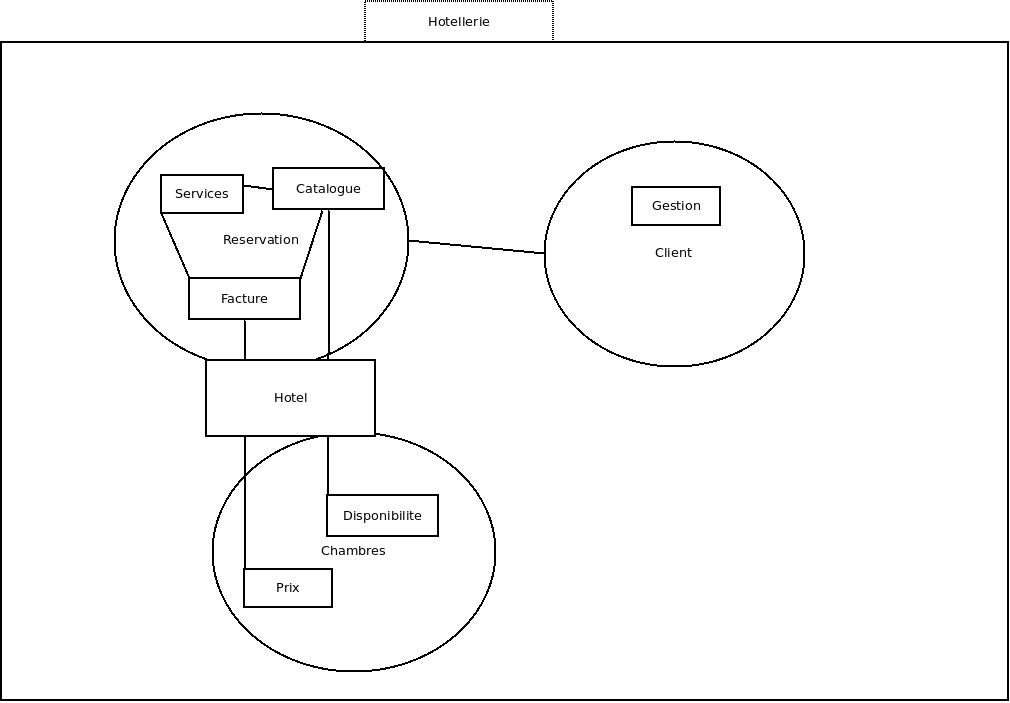
\includegraphics[width=10cm]{ddd.png} \\


\subsection{Ajout/Suppression d'un client}
Cette fonctionnalit\'e est bien \'evidemment indispensable.

\subsection{Modification du prix}
Il serait \'egalement int\'eressant d'avoir la possibilit\'e de pouvoir modifier les prix pour les m\^{e}mes raisons que cit\'ees plus.


\subsection{\'Etat des chambres}
Il faudrait savoir quelles chambres sont disponibles. Il faudrait \'egalement pouvoir modifier l\'etat des chambres (libre ou occup\'ee). Il faudrait aussi savoir combien de chambres sont disponibles (par h\^{o}tel).

\subsection{R\'eservation}
Il faut bien s\^{u}r pouvoir modifer (ajout/suppression) les r\'eservations. On pourrait donc bien s\^{u}r pouvoir  avoir acc\`es au calendrier.


\subsection{Ajout/suppression de chambres}
Il serait int\'eressant de pouvoir ajouter ou supprimer des chambres si l'h\^{o}tel subbit des modifications physiques.


\subsection{Ajout/suppression d'h\^{o}tels}
Il serait, comme pour les chambres, \'egalement int\'eressant de pouvoir supprimer ou ajouter des h\^{o}tels si n\'ecessaire.


\subsection{Mail}
Permettrait de pouvoir \'ecrire des mails.

\pagebreak
\begin{landscape}
\section{Microservices}
	\centering
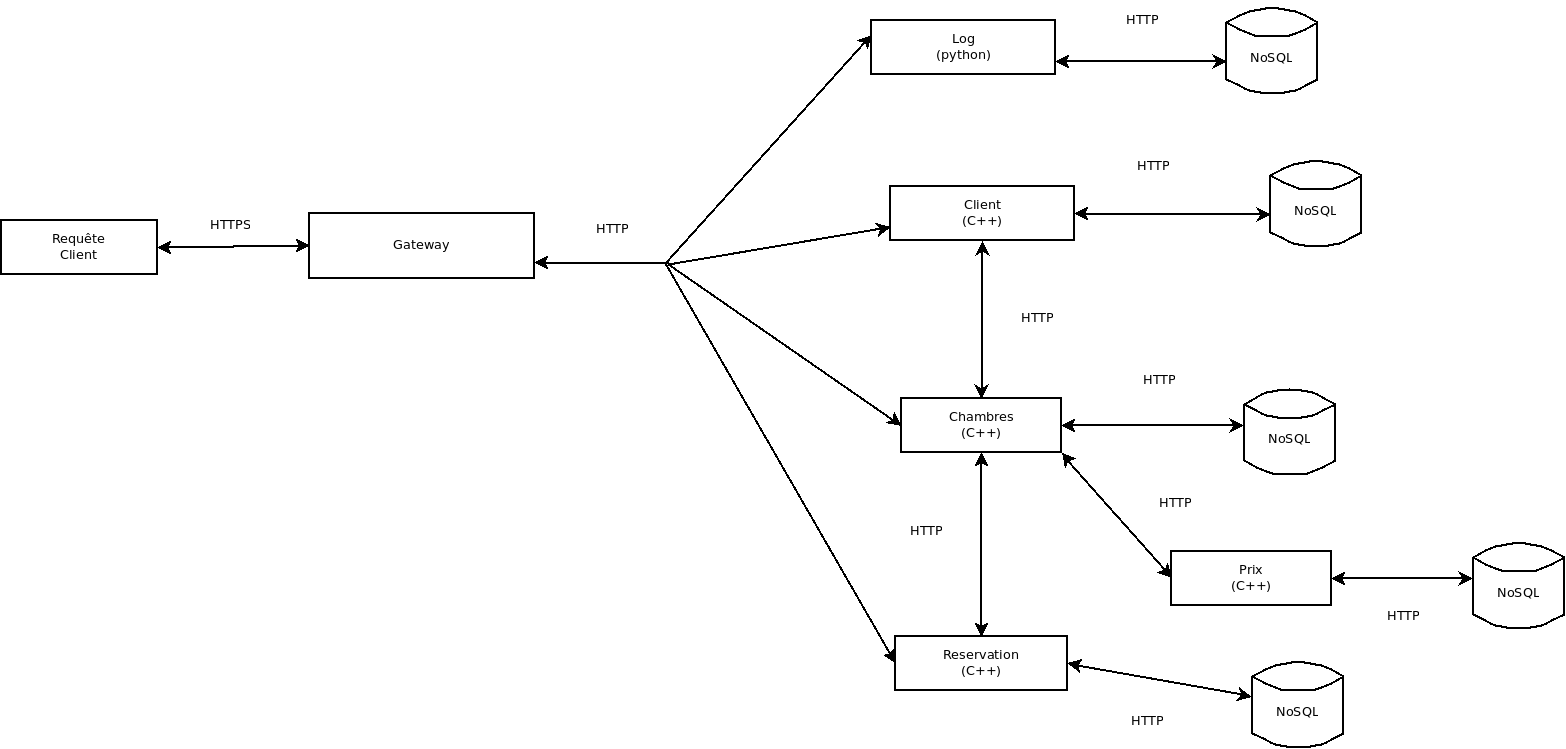
\includegraphics[width=18cm]{microservices.png} \\
\end{landscape}

\pagebreak
\vspace{1cm}
Le pattern utilis\'e serait avec simplement un gateway/aggregator qui permettrait de pouvoir faire appel aux diff\'erents services, soit de pouvoir modifer/r\'ecup\'erer des donn\'ees. Si un service a besoin de faire appel \`a un autre, il passerait par la gateway. La communication se fera gr\^{a}ce \`a l'API REST.

\subsection{Log}
Ce service permet d'avoir un syst\`eme de logs. Pensant faire tourner les serveurs sous linux, les logs seraient sauvegard\'es sous \begin{verbatim} /var/log/<type de service> \end{verbatim}
\leavevmode \linebreak[3]
Avec, par exemple, \textit{$<$type de service$>$} :
\begin{itemize}
	\item syst\`eme
	\item communication entre les microservices
\end{itemize}


\subsection{Client}
Ce service permettrait d'\'{e}crire et de lire dans la base de donn\'ees des clients.

\subsection{R\'eservation}
Ce service permettrait d'\'{e}crire et de lire dans la base de donn\'ees des r\'eservations.


\subsection{Prix}
Puisque les prix fluctuent en fonction du jour, ce service permettrait de r\'ecup\'erer le prix actuel.


\subsection{R\'ecup\'eration de log}
Ce service permettrait de pouvoir lire les logs.

\subsection{Chambres}
Ce service permettrait de pouvoir lire et \'ecrire dans la base de donn\'ees des chambres.

\pagebreak
\section{Routes}
\begin{itemize}

	\item GET
	\begin{itemize}
	\item /client/lname/\{lname\}/fname/\{fname\}/mail/\{mail\}\\
		R\'ecup\`ere l'id d'un client \\
		\textit{lname}: string \\
		\textit{fname}: string \\
		\textit{mail}: string \\
		retourne: int

	\item /hotels\\
		R\'ecup\`ere tous les h\^{o}tels \\
		retourne: int[]

	\item /client/id/\{id\}\\
		R\'ecup\`ere un client sp\'ecifique \\
		\textit{id}: int \\
		retourne: dictionnaire

	\item /room/id/\{id\}\\
		R\'ecup\`ere une chambre\\
		\textit{id}: int \\
		retourne: dictionnaire

	\item /hotel/id/\{id\}/rooms\\
		R\'ecup\`ere toutes les chambres d'un h\^{o}tel\\
		\textit{id}: int \\
		retourne: int[]

	\item /hotel/id/\{hotel\_id\}/room/id/\{room\_id\}\\
		R\'ecup\`ere la chambre d'un h\^{o}tel \\
		\textit{hotel\_id}: int \\
		\textit{room\_id}: int \\
		retourne: dictionnaire

	\item /calendar\\
		R\'ecup\`ere le calendrier \\
		retourne: dictionnaire

	\item /calendar/year/\{year\}\\
		R\'ecup\`ere le calendrier mais pour une seule ann\'ee \\
		retourne: dictionnaire

	\item /booking/id/\{booking\_id\}/client/\{client\_id\}\\
		R\'ecup\`ere une r\'eservation pour un client \\
		\textit{booking\_id}: int \\
		\textit{client\_id}: int \\
		retourne: dictionnaire

	\item /booking/day/\{day\}/month/\{month\}/year/\{year\}/nights/\{nights\} \\
		R\'ecup\`ere les chambres libres pour la date et le nombre de nuits indiqu\'es \\
		\textit{day}: int \\
		\textit{month}: int \\
		\textit{year}: int \\
		\textit{nights}: int \\
		retourne: int[]

	\item /room/\{id\}/price \\
		R\'ecup\`ere le prix d'une chambre \\
		\textit{id}: int \\
		retourne: int

	\item /service/id/\{id\}/price \\
		R\'ecup\`ere le prix d'un service \\
		\textit{id}: int \\
		retourne: int

	\item /booking/id/\{id\}/service \\
		R\'ecup\`ere les services d'une r\'eservation \\
		\textit{id}: int \\
		retourne: int[]
	\end{itemize}

\item UPDATE
	\begin{itemize}

		\item /client/id/\{id\}/fname/\{fname\}\\
		Met \`a jour le pr\'enom d'un client \\
		\textit{id}: int \\
		\textit{fname}: string


	\item /client/id/\{id\}/lname/\{lname\}\\
		Met \`a jour le nom de famille d'un client \\
		\textit{id}: int \\
		\textit{lname}: string

	\item /client/id/\{id\}/mail/\{mail\}\\
		Met \`a jour le mail d'un client \\
		\textit{id}: int \\
		\textit{mail}: string

	\item /booking/id/\{id\}/state/\{state\} \\
		Met \`a jour la r\'eservation \\
		\textit{id}: int \\
		\textit{state}: int

	\item /room/id/\{id\}/roomtype/\{rtype\_id\} \\
		Met \`a jour une chambre \\
		\textit{id}: int \\
		\textit{rtype\_id}: int

	\item /room/id/\{id\}/price/\{price\} \\
		Modifie le prix d'une chambre \\
		\textit{id}: int \\
		\textit{price}: int \\
	\end{itemize}

\item POST
	\begin{itemize}

		\item /client/lname/\{lname\}/fname/\{fname\}/mail/\{mail\}\\
		Ajoute un client \\
		\textit{lname}: string \\
		\textit{fname}: string \\
		\textit{mail}: string

	\item /room/roomtype/\{rtype\_id\}\\
		Ajoute une nouvelle chambre \\
		\textit{rtype\_id}: int

	\item /booking/day/\{day\}/month/\{month\}/year/\{year\}/nights/\{nights\}/room/id/\{room\_id\}- /client/id/\{client\_id\}\\
		Ajoute une r\'eservation \\
		\textit{day}: int \\
		\textit{month}: int \\
		\textit{year}: int \\
		\textit{nights}: int \\
		\textit{room\_id}: int \\
		\textit{client\_id}: int

	\item /hotel/id/\{id\}\\
		ajoute un nouvel h\^{o}tel \\
		\textit{id}: int

	\item /booking/id/\{booking\_id\}/service/id/\{service\_id\} \\
		Ajoute un service \`a une r\'eservation \\
		\textit{booking\_id}: int \\
		\textit{service\_id}: int
	\end{itemize}

\item DELETE
	\begin{itemize}
	\item /client/id/\{id\}\\
		Supprime un client \\
		\textit{id}: int

	\item /booking/id/\{id\}\\
		Supprime une r\'eservation \\
		\textit{id}: int

	\item /hotel/id/\{id\}\\
		Supprime un h\^{o}tel \\
		\textit{id}: int

	\item /room/id/\{id\}\\
		Supprime une chambre \\
		\textit{id}: int

	\item /service/id/\{id\}\\
		Supprime un service \\
		\textit{id}: int

	\end{itemize}
\end{itemize}


\end{document}
